\documentclass[12pt]{report}
\usepackage[utf8]{inputenc}
\usepackage{graphicx}
\usepackage{amsmath}
\usepackage{hyperref}
\usepackage{makecell}
\usepackage{adjustbox}
\usepackage{geometry} 
\usepackage{subcaption}
\usepackage{float}

\title{Assignment 3: \\ Unsupervised learning with
	PCA, t-SNE, k-means, AHC and SOM\\ Neuronal and evolutionary computing\\ 2023 - 2024}
\author{Pawel Puzdrowski}
\date{2023-12-17}

\begin{document}
	\maketitle
	\section*{Part 1}
	\subsection*{Dataset1 - provided from course site}
	No changes to column values were made to the first dataset, only z-score normalization was done on the columns except the last one (class column) with simple jupyter notebook "dataCleaningNotebooks.ipynb" which is situated in directory "DataCleaning". The file for this dataset is in directory "datasets" and the name is "A3-dataset1Modified.csv". 
	\subsection*{Dataset from internet - Dry bean dataset}
	The second dataset was obtained from the kaggle.com website specifically \cite{DatasetDryBeans}. This website consists of 16 variables, one class column and 2501 features. The database represents data that was obtained from a computer vision system where seven different dry beans were examined by a high resolution camera and over 13 000 images were taken. The website provides two csv files, one for testing and one for training, only the training csv file is used because the criterium for this task that the dataset needs to have at least 200 features and the training csv file has 2500 features which is enough. \\
	\\
	This dataset class column values are categorical values (text) which represents different beans. There exist seven different beans names and they were changed for numbers. How the bean names were changes in the class column is shown in table \ref{BeanClassChange}. Z-score normalization was applied to every column because the columns had a lot of outliers, the last column, class, was not normalized. The modification and normalization was done with script "dataCleaningNotebooks.ipynb" which is in directory "DataCleaning". 
	\begin{table}[H]
		\centering
		\begin{tabular}{|c|c|}
			\hline
			Old value & New value  \\
			\hline
			SEKER & 0 \\
			\hline
			BARBUNYA & 1 \\
			\hline
			BOMBAY & 2 \\
			\hline
			CALI & 3 \\
			\hline
			DERMASON & 4 \\
			\hline
			HOROZ & 5 \\
			\hline
			SIRA & 6 \\
			\hline
		\end{tabular}
		\caption{Bean names change}
		\label{BeanClassChange}
	\end{table}
	\newpage
	\section*{Part 2}
	\subsection*{PCA}
	Implementation of PCA is situated in directory "PCA" where a jupyter notebook file exist, "PCA.ipynb". \\
	\\
	Scatter plot and scree plot for dataset 1 is visualized in figure \ref{Dataset1scatterPlot} and \ref{Dataset1ScreePlot} respectively. Plot for dataset2 is visualized
	in figure \ref{Dataset2scatterPlot} and \ref{Dataset2ScreePlot}.\\
	\\
	The PCA doesn't do a good job in classifying the different classes in dataset 1. The scatter plot is spread over the graph and it's hard to see the clusters. Scatter plot for dataset 2 on the other hand is much better and the clusters are visible.\\
	\\
	\textbf{Dataset1}\\
	\begin{figure}[H]
		\centering
		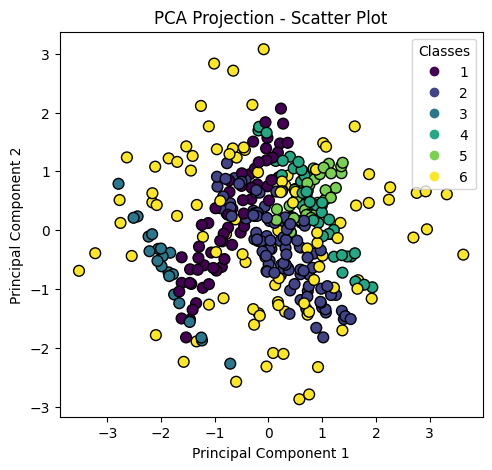
\includegraphics[width=0.5\textwidth]{../PCA/OutputPlot/Dataset1/Dataset1scatterPlot.png}
		\caption{Dataset1 scatter plot}
		\label{Dataset1scatterPlot}
	\end{figure}
	\begin{figure}[H]
		\centering
		\includegraphics[width=0.5\textwidth]{../PCA/OutputPlot/Dataset1/Dataset1ScreePlot.png}
		\caption{Dataset1 scree plot}
		\label{Dataset1ScreePlot}
	\end{figure}

	\textbf{Dataset2}\\
	\begin{figure}[H]
		\centering
		\includegraphics[width=0.5\textwidth]{../PCA/OutputPlot/Dataset2/Dataset2scatterPlot.png}
		\caption{Dataset2 scatter plot}
		\label{Dataset2scatterPlot}
	\end{figure}
	\begin{figure}[H]
		\centering
		\includegraphics[width=0.5\textwidth]{../PCA/OutputPlot/Dataset2/Dataset2ScreePlot.png}
		\caption{Dataset2 scree plot}
		\label{Dataset2ScreePlot}
	\end{figure}

	\newpage
	\subsection*{t-SNE}
	Documentation for t-SNE in python was accessed by the official scikit learn website \cite{Doct-SNE}. According to the documentation the important parameters that can be tuned are following:
	\begin{itemize}
		\item perplexity - values should be between 5 and 50. Is connected to number of nearest neighbours, for bigger datasets this parameter should be bigger.
		\item learning$\_$rate - How fast the model classifies the data, the value for this parameter is given by: $\frac{\frac{Number of samples}{early\_exaggeration}}{4}$
		\item n$\_$iter - number of iteration
	\end{itemize}
	Other parameters in t-SNE have either value "None" or have no impact on the classification if the parameter changes. These are the other paramters:
	\begin{itemize}
		\item early$\_$exaggeration - value: the program changes this parameter auomatically.\\
		Defines how much space will be between clusters
		\item n$\_$components - value: default=2\\
		sets the dimension of embedded space, the task description says that the t-SNE projection should be found in 2D.
		\item n$\_$iter$\_$without$\_$progress - value: default=300\\
		Maximum number of iterations without progress. Decreasing and increasing the value doesn't affect the output plot.
		\item min$\_$grad$\_$norm - value: default=1e-7\\
		Decreasing and increasing the value doesn't affect the output plot.
		\item metric - default=’euclidean’\\
		Method to calculate the distance between points, other methods have no change in the output plot.
		\item metric$\_$params - value: default=None\\
		Additional keyword arguments for the metric function. Hard to find other specification for this parameter
		\item init - value: default=”pca”\\
		Other value for this paramter is "random" and it spreads out the clusters and changes the value so the output plot is not better.
		\item verbose - value: 1\\
		If set to 1, gives more information what happens at every step of the iterations.
		\item random$\_$state - value: default=None\\
		Randomize the data, doesn't have an effect on the output plot.
		\item method - value: default=’barnes$\_$hut’\\
		Gradient calculation algorithm. The other option for this parameter is "exact", the program is slower and doesn't show any improvement in the output plot.
		\item angle - value: default=0.5\\
		According to the documentation, this variable doesn't have big effect on the output.
		\item n$\_$jobs - value: default=None\\
		Parallelization of the program. Not relevant for this assignment.
	\end{itemize}
	\textbf{Dataset 1}
	\begin{table}[H]
		\centering
		\begin{tabular}{|c|c|c|c|c|c|c|}
			\hline
			Dataset1 & Test 1 & Test 2 & Test 3 & Test 4 & Test 5& optimal values \\
			\hline
			Perplexity & 20 & 5 & 5 & 5 & 20 & 5 \\
			\hline
			Learning$\_$rate & 2 & 30 & 2 & 5 & 30 & 2 \\
			\hline
			n$\_$iter & 1000 & 1000 & 1500 & 500 & 1000 & 1000 \\
			\hline
		\end{tabular}
		\caption{Dataset 1 parameter values}
		\label{dataset1ParameterValues}
	\end{table}
	The different values for t-SNE parameters are shown in table \ref{dataset1ParameterValues}, five columns are for test values and one column for optimal values for dataset 1. The output plot from this tests are visualized in the following figures:\\
	\\
	\begin{itemize}
		\item Increased perplexity - figure \ref{dataset1IncreasedPerplexity}
		\item Increased learning rate - figure \ref{Dataset1IncreasedLearning}
		\item Increased and decreased number of iterations - figure \ref{Dataset1IncreasedDecreasedNrIterations}
		\item Increased both learning rate and perplexity - figure \ref{dataset1IncreasedLearningANDPerplexity}
	\end{itemize}
	The output plot from the optimal parameter values is shown in figure \ref{dataset1OptimalparameterValuesPlot}. Perplexity was chosen to be the lowest value 5, because the dataset 1 is a small database and according to documentation the value for this parameter should be small with small datasets. Learning rate value is obtain by the following equation: \\
	\\
	$\frac{\frac{Number of samples}{early\_exaggeration}}{4}$\\
	\\
	early$\_$exaggeration is chosen automatically by the program and the value was 61 and the final learning rate was calculated to be:\\
	\\
	$\frac{\frac{361}{61}}{4} \approx 2$\\
	\\
	Number of iteration was set to 1000, increasing or decreasing it more didn't give better output, according to figure \ref{Dataset1IncreasedDecreasedNrIterations}.\\
	\\
	The t-SNE program seems to do a pretty good job in clustering almost all data points except the class 6 datapoints. Wasn't able to find parameter values that could handle all classes including the sixth one. 
	\newpage
	\begin{figure}[H]
		\centering
		\begin{subfigure}{.5\textwidth}
			\centering
			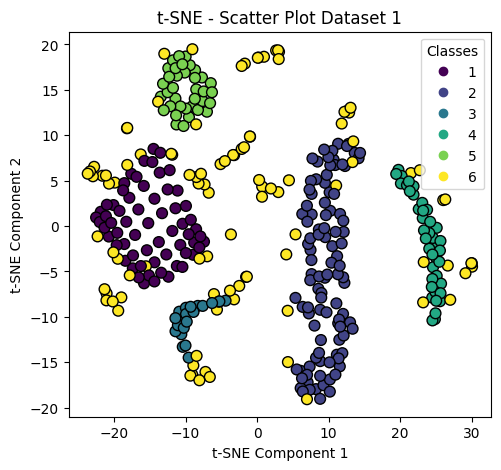
\includegraphics[width=.8\linewidth]{../t-SNE/OutputPlot/Dataset1OutputPlot/Dataset1 increased learningRate.png}
			\caption{Increased learning rate}
			\label{Dataset1IncreasedLearning}
		\end{subfigure}%
		\begin{subfigure}{.5\textwidth}
			\centering
			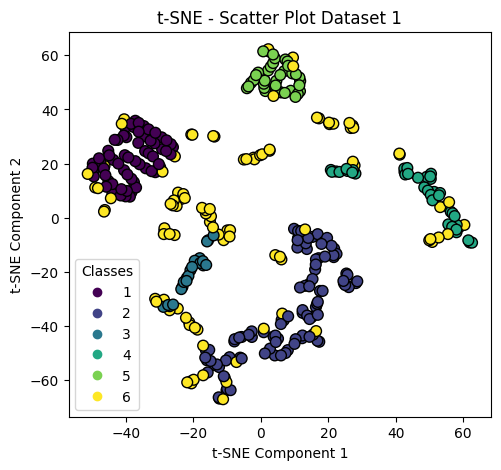
\includegraphics[width=.8\linewidth]{../t-SNE/OutputPlot/Dataset1OutputPlot/Dataset1 increased perplexity.png}
			\caption{Increased perplexity}
			\label{dataset1IncreasedPerplexity}
		\end{subfigure}
		\caption{Output plot for increased learning rate and perplexity for dataset 1}
		\label{Dataset1IncreasedLearningperplexity}
	\end{figure}
	\begin{figure}[H]
		\centering
		\begin{subfigure}{.5\textwidth}
			\centering
			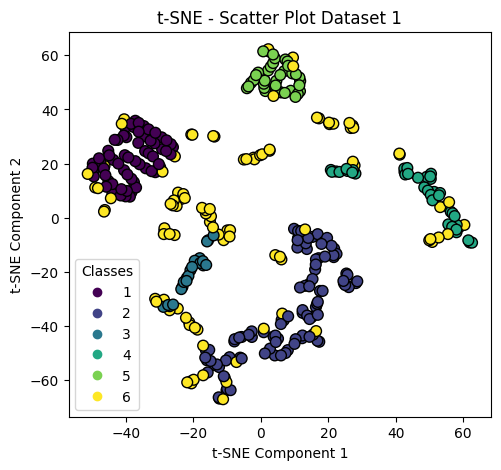
\includegraphics[width=.8\linewidth]{../t-SNE/OutputPlot/Dataset1OutputPlot/Dataset1 increased nr_plots.png}
			\caption{Increased number of iterations}
			\label{Dataset1IncreasedNrIterations}
		\end{subfigure}%
		\begin{subfigure}{.5\textwidth}
			\centering
			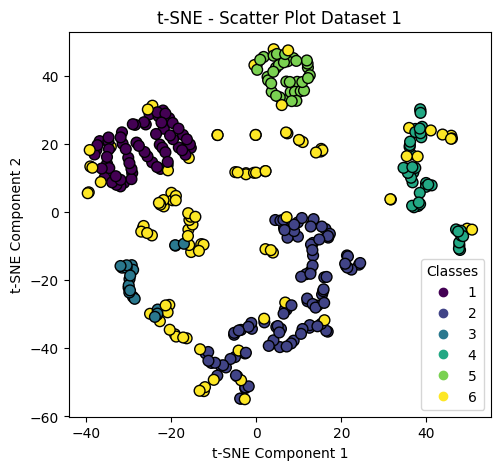
\includegraphics[width=.8\linewidth]{../t-SNE/OutputPlot/Dataset1OutputPlot/Dataset1 decreased nr_plots.png}
			\caption{Decreased number of iterations}
			\label{Dataset1DecreasedNrIterations}
		\end{subfigure}
		\caption{Increased and decreased number of iterations output plot}
		\label{Dataset1IncreasedDecreasedNrIterations}
	\end{figure}
	\begin{figure}[H]
		\centering
		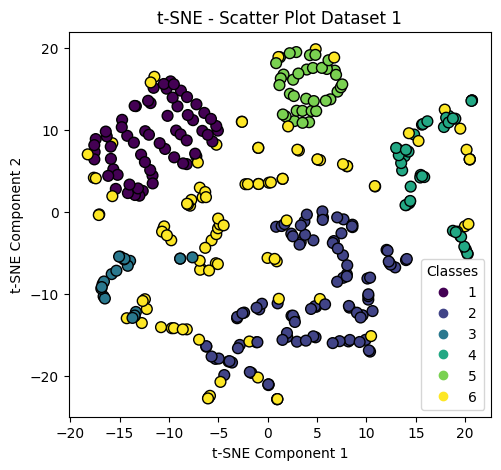
\includegraphics[scale=0.7]{../t-SNE/OutputPlot/Dataset1OutputPlot/Dataset1 increased learning and perplexity.png}
		\caption{Dataset 1 increased learning rate and perplexity}
		\label{dataset1IncreasedLearningANDPerplexity}
	\end{figure}
	\begin{figure}[H]
		\centering
		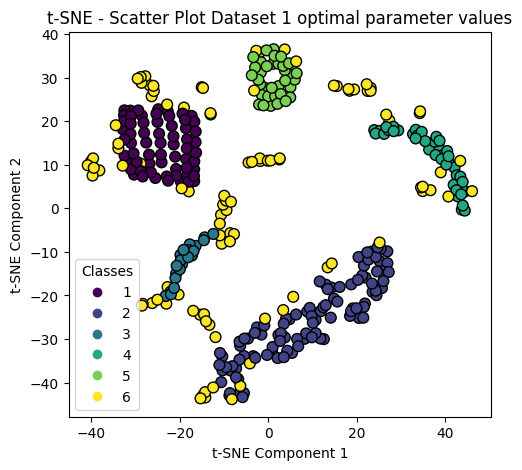
\includegraphics[scale=0.7]{../t-SNE/OutputPlot/Dataset1OutputPlot/dataset1 optimal parameter values.png}
		\caption{Dataset 1 optimal parameter values plot}
		\label{dataset1OptimalparameterValuesPlot}
	\end{figure}
	\newpage
	\textbf{Dataset 2 - dry beans}\\
	The different parameter values that were tested are shown in table \ref{dataset2ParameterValues}. \\
	\\
	All the parameter values gave almost the same output plot of the different classes, the best one was the one with perplexity 30, learning rate 10 and number of iterations 1000, which is shown in figure \ref{dataset2optimalValues} but can even say that the perplexity: 50 was good as well. The worst was the one with perplexity 20 because the clusters are more spread.\\
	\\
	As shown in figure \ref{Dataset2Diffnr_iter}, number of iteration has a slightly influence on the clusterring. Figure \ref{Dataset2Diffnr_perplexity} shows different tests with different values for perplexity and for this dataset higher value for perplexity seems to be an advantage. Learning rate on the other hand, as shown in figure \ref{Dataset2DiffLearningRate}, doesn't have big effect on the t-SNE output.\\
	\\
	The optimal values where obtained as follows:\\
	Learning rate, as in the previous dataset, was obtained by this equation:\\
	\\
	$\frac{\frac{Number of samples}{early\_exaggeration}}{4}$\\
	\\
	The value for optimal learning was calculated to be:\\
	\\
	$\frac{\frac{2500}{68}}{4} \approx 10$\\
	\\
	The perplexity was set to be higher than for the dataset 1 because dataset 2 is larger and perplexity should be larger when database increases. Number of iterations was set to 1000 because increasing more didn't give any better output plot.\\
	\newpage
	
	\begin{table}[H]
		\centering
		\begin{tabular}{|c|c|c|c|c|c|c|c|c|}
			\hline
			Dataset1 & Test 1 & Test 2 & Test 3 & Test 4 & Test 5 & Test 6 & Test 7& Optimal values \\
			\hline
			Perplexity & 20 & 35 & 50 & 30 & 30 & 30 & 30 & 30 \\
			\hline
			Learning$\_$rate & 10 & 10 & 10 & 30 & 100 & 10 & 10 & 10 \\
			\hline
			n$\_$iter & 1000 & 1000 & 1000 & 1000 & 1000 & 500 & 1500 & 1000 \\
			\hline
		\end{tabular}
		\caption{Dataset 2 parameter values}
		\label{dataset2ParameterValues}
	\end{table}
	
	\begin{figure}[H]
		\centering
		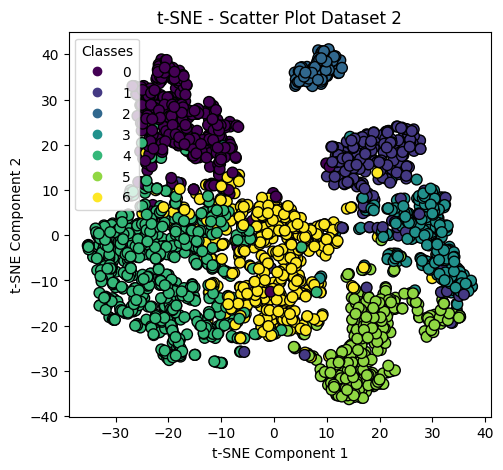
\includegraphics[scale=0.7]{../t-SNE/OutputPlot/Dataset2Outputplot/OptimalValues.png}
		\caption{Dataset 2 optimal values: perplexity: 30, learningRate: 10, nIter: 1000}
		\label{dataset2optimalValues}
	\end{figure}

	\begin{figure}[H]
		\centering
		\begin{subfigure}{.5\textwidth}
			\centering
			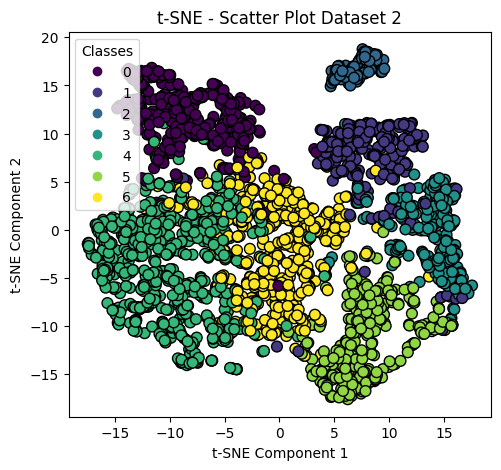
\includegraphics[width=.8\linewidth]{../t-SNE/OutputPlot/Dataset2Outputplot/n_iter500.png}
			\caption{Number of iteration: 500}
			\label{Dataset2nr_iter500}
		\end{subfigure}%
		\begin{subfigure}{.5\textwidth}
			\centering
			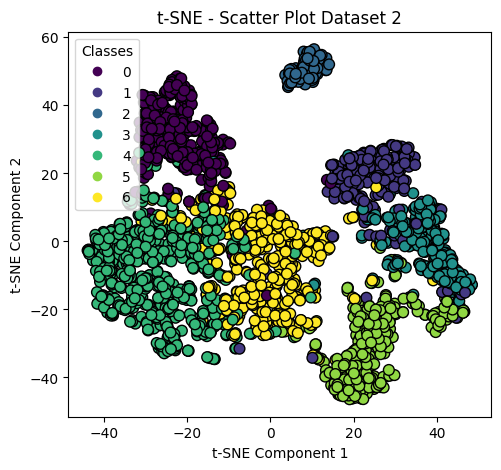
\includegraphics[width=.8\linewidth]{../t-SNE/OutputPlot/Dataset2Outputplot/n_iter1500.png}
			\caption{Number of iteration: 1500}
			\label{Dataset2nr_iter1500}
		\end{subfigure}
		\caption{Database 2: Different number of iterations with perplexity: 30, learningRate: 10}
		\label{Dataset2Diffnr_iter}
	\end{figure}

	\begin{figure}[H]
		\centering
		\begin{subfigure}{.33\textwidth} % Adjust the width if necessary
			\centering
			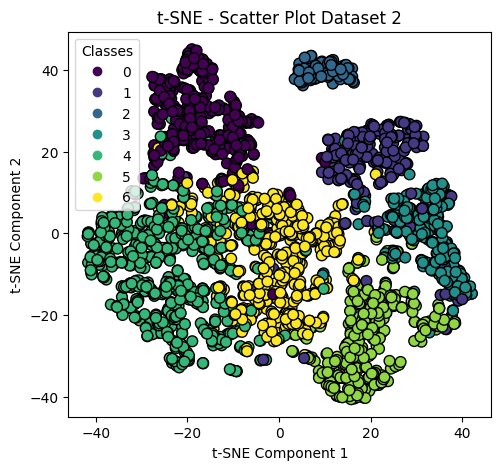
\includegraphics[width=\linewidth]{../t-SNE/OutputPlot/Dataset2Outputplot/perplexity20.png}
			\caption{Perplexity = 20}
			\label{Dataset2perplexity20}
		\end{subfigure}%
		\begin{subfigure}{.33\textwidth} % Adjust the width if necessary
			\centering
			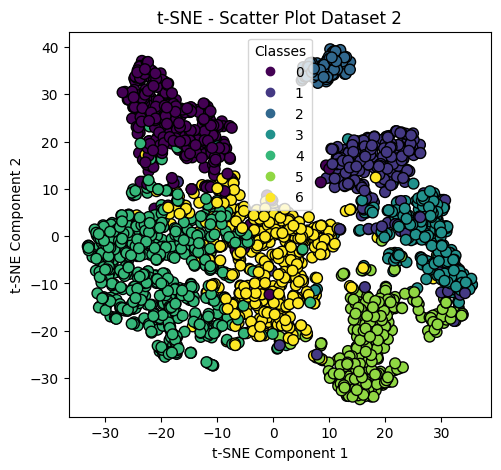
\includegraphics[width=\linewidth]{../t-SNE/OutputPlot/Dataset2Outputplot/perplexity35.png}
			\caption{Perplexity: 35}
			\label{Dataset2perplexity35}
		\end{subfigure}%
		\begin{subfigure}{.33\textwidth} % Adjust the width if necessary
			\centering
			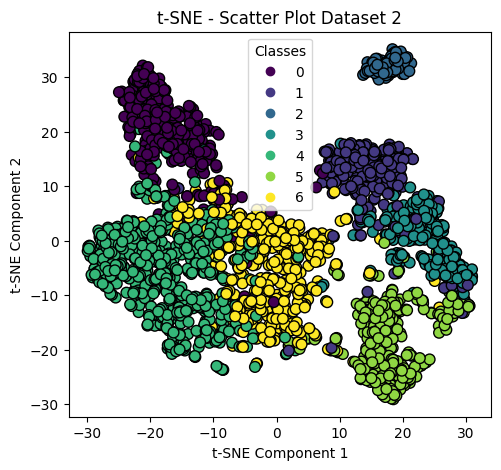
\includegraphics[width=\linewidth]{../t-SNE/OutputPlot/Dataset2Outputplot/perplexity50.png}
			\caption{Perplexity: 50}
			\label{Dataset2perplexity50}
		\end{subfigure}
		\caption{Database 2: Different perplexities, learningRate: 10, nr$\_$iter = 1000}
		\label{Dataset2Diffnr_perplexity}
	\end{figure}

	\begin{figure}[H]
		\centering
		\begin{subfigure}{.5\textwidth}
			\centering
			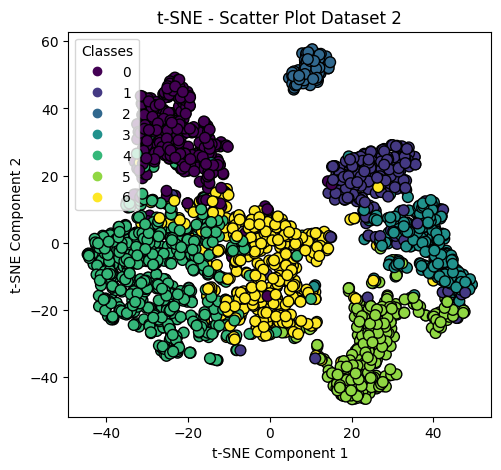
\includegraphics[width=.8\linewidth]{../t-SNE/OutputPlot/Dataset2Outputplot/perplexity30learningrate30.png}
			\caption{learningRate: 30}
			\label{Dataset2LearningRate30}
		\end{subfigure}%
		\begin{subfigure}{.5\textwidth}
			\centering
			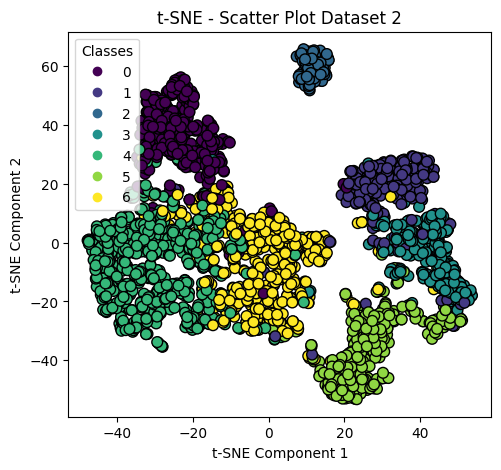
\includegraphics[width=.8\linewidth]{../t-SNE/OutputPlot/Dataset2Outputplot/perplexity30learningrate100.png}
			\caption{learningRate: 100}
			\label{Dataset2LearningRate100}
		\end{subfigure}
		\caption{Database 2: Different learningRate, perplexity:30, nr$\_$iter = 1000}
		\label{Dataset2DiffLearningRate}
	\end{figure}
	\newpage
	\subsection*{k-means}
	\textbf{Dataset 1:}\\
	\\
	Script for k-means, k-means.ipynb, algorithm is situaited in directory "K-means".\\
	\\
	To get the optimal values for k, elbow method was used as describe in this source \cite{k-means}. The optimal value for k is 4 for dataset 1 because according to the elbow method plot in figure \ref{dataset1ElobowMethod}, the "elbow" appears when k = 4. Because the datasets has more than two features, the datasets were dimensionally reduced with PCA. \\
	\\
	As an additional evaluation of the k-means performance ARI (Adjusted Rand Index) and NMI (Normalized Mutual Information) scores was used. These scores ranges between 0 and 1 where 0 means worst classification and 1 means perfect classification. The ARI and NMI scores are shown in table \ref{dataset1k-meansARINMI}.\\
	\\
	For dataset 1 this set of k values was used: 2, 3, 4, 5, 6. The output from the program is visualized in the following plots:
	\begin{itemize}
		\item k = 2,3 scatter plot: figure \ref{Dataset1Scatterplot23}, confusion matrix plot: figure \ref{Dataset1ConfussionMatrix23} 
		\item k = 4,5,6 scatter plot: figure \ref{Dataset1Scatterplot456}, confusion matrix plot: figure \ref{Dataset1ConfussionMatrix456}
	\end{itemize}
	K-means method is not doing a good job in clustering the data. Scatter plots for all k values contains very spread data and the ARI and NMI values doesn't improve when k is increased. Confusion matrix is showing a lot of values that are not classified correctly, the diagonal of every confusion matrix has small values which means that the model is not able to classify the data correctly.
	\begin{table}[H]
		\centering
		\begin{tabular}{|c|c|c|}
			\hline
			K & ARI & NMI \\
			\hline
			2 & 0.196 & 0.345 \\
			\hline
			3 & 0.280 & 0.416 \\
			\hline
			4 & 0.225 & 0.408 \\
			\hline
			5 & 0.228 & 0.406 \\
			\hline
			6 & 0.230 & 0.408 \\
			\hline
		\end{tabular}
		\caption{Dataset 1 k-means ARI and NMI values}
		\label{dataset1k-meansARINMI}
	\end{table}
	\newpage
	\textbf{Dataset 2:}\\
	\\
	For dataset 2 this set of k values was used: 2, 3, 4, 5, 6, 7, 8. The output is visualized in the following plots:
	\begin{itemize}
		\item k = 2,3 scatter plot: figure \ref{Dataset2Scatterplot23}, confusion matrix plot: figure \ref{Dataset2ConfussionMatrix23} 
		\item k = 4,5,6 scatter plot: figure \ref{Dataset2Scatterplot456}, confusion matrix plot: figure \ref{Dataset2ConfussionMatrix456}
		\item k = 7,8 scatter plot: figure \ref{Dataset2Scatterplot78}, confusion matrix plot: figure \ref{Dataset2ConfussionMatrix78}
		\item Elbow method plot \ref{dataset2ElobowMethod}	
	\end{itemize}
	For the dataset 2, k-means is doing a better job than for dataset 1. The plot from elbow method says that the optimal value for k is 6 and it is even visible on the ARI and NMI score in table \ref{Dataset2ARIMNI} that the ARI and NMI scores increase until k is equal to 6 and further increase, decreases the scores. Scatter plot for k = 6 shows clear clusters and confusion matrix for the same k value has a decent amount of values on the diagonal cells.
	\begin{table}[H]
		\centering
		\begin{tabular}{|c|c|c|}
			\hline
			K & ARI & NMI \\
			\hline
			2 & 0.0352 & 0.1695 \\
			\hline
			3 & 0.3030 & 0.4987 \\
			\hline
			4 & 0.3945 & 0.5990 \\
			\hline
			5 & 0.5597 & 0.6960 \\
			\hline
			6 & 0.6849 & 0.7327 \\
			\hline
			7 & 0.6661 & 0.7113 \\
			\hline
			8 & 0.5612 & 0.6646 \\
			\hline
		\end{tabular}
		\caption{Dataset 2: ARI and NMI Scores for Different Values of K}
		\label{Dataset2ARIMNI}
	\end{table}
	

	\begin{figure}[H]
		\centering
		\begin{subfigure}{.5\textwidth}
			\centering
			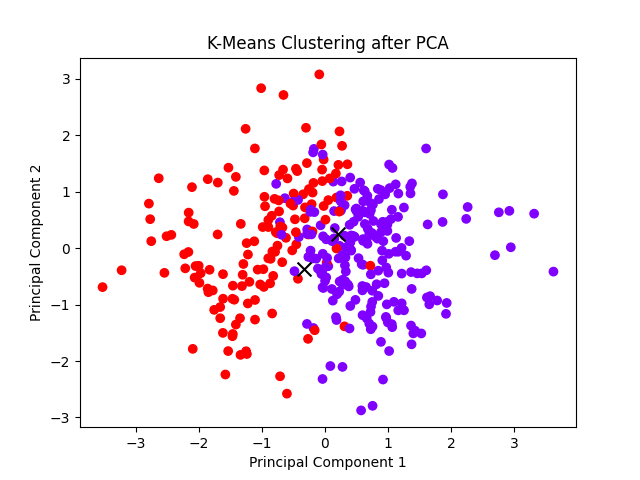
\includegraphics[width=.9\linewidth]{../K-means/Output/Dataset1/scatterPlot_k=2.png}
			\caption{Scatter plot for k = 2}
			\label{Dataset1Scatterplotk2}
		\end{subfigure}%
		\begin{subfigure}{.5\textwidth}
			\centering
			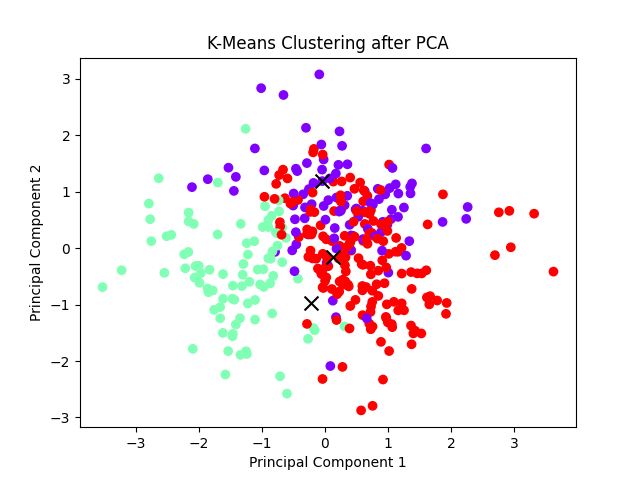
\includegraphics[width=.9\linewidth]{../K-means/Output/Dataset1/scatterPlot_k=3.png}
			\caption{Scatter plot for k = 3}
			\label{Dataset1Scatterplotk3}
		\end{subfigure}
		\caption{Dataset 1: Scatter plot with value k = 2,3}
		\label{Dataset1Scatterplot23}
	\end{figure}

	\begin{figure}[H]
		\centering
		\begin{subfigure}{.5\textwidth}
			\centering
			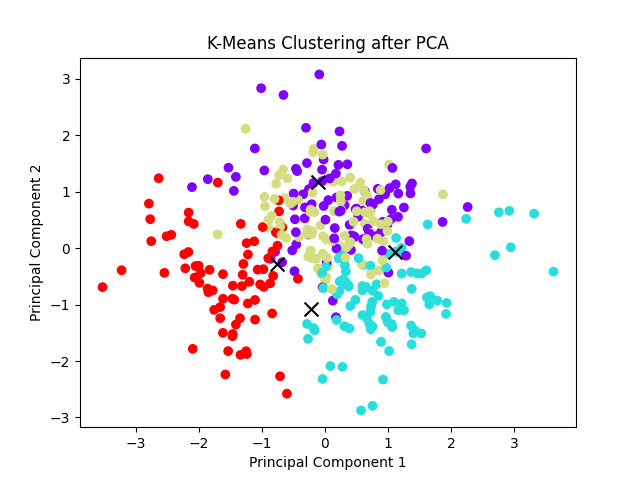
\includegraphics[width=.9\linewidth]{../K-means/Output/Dataset1/scatterPlot_k=4.png}
			\caption{Scatter plot for k = 4}
			\label{Dataset1Scatterplotk4}
		\end{subfigure}%
		\begin{subfigure}{.5\textwidth}
			\centering
			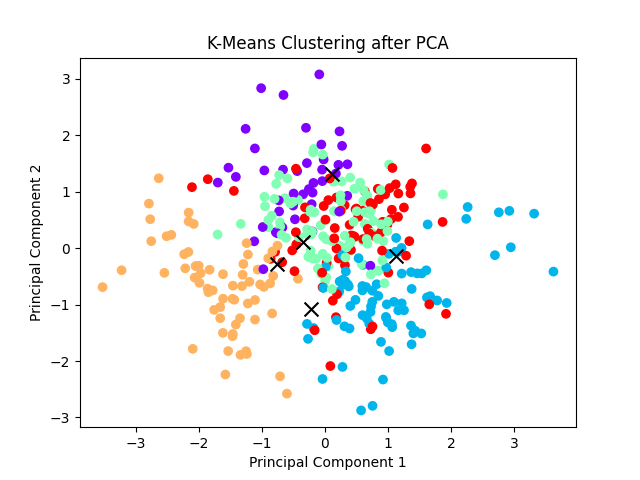
\includegraphics[width=.9\linewidth]{../K-means/Output/Dataset1/scatterPlot_k=5.png}
			\caption{Scatter plot for k = 5}
			\label{Dataset1Scatterplotk5}
		\end{subfigure}
		\begin{subfigure}{.5\textwidth}%
			\centering
			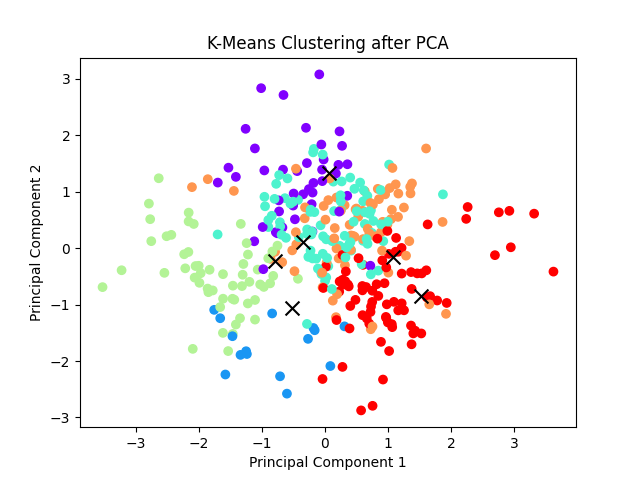
\includegraphics[width=.9\linewidth]{../K-means/Output/Dataset1/scatterPlot_k=6.png}
			\caption{Scatter plot for k = 6}
			\label{Dataset1Scatterplotk6}
		\end{subfigure}
		\caption{Dataset 1: Scatter plot with value k = 4, 5, 6}
		\label{Dataset1Scatterplot456}
	\end{figure}

	\begin{figure}[H]
		\centering
		\begin{subfigure}{.5\textwidth}
			\centering
			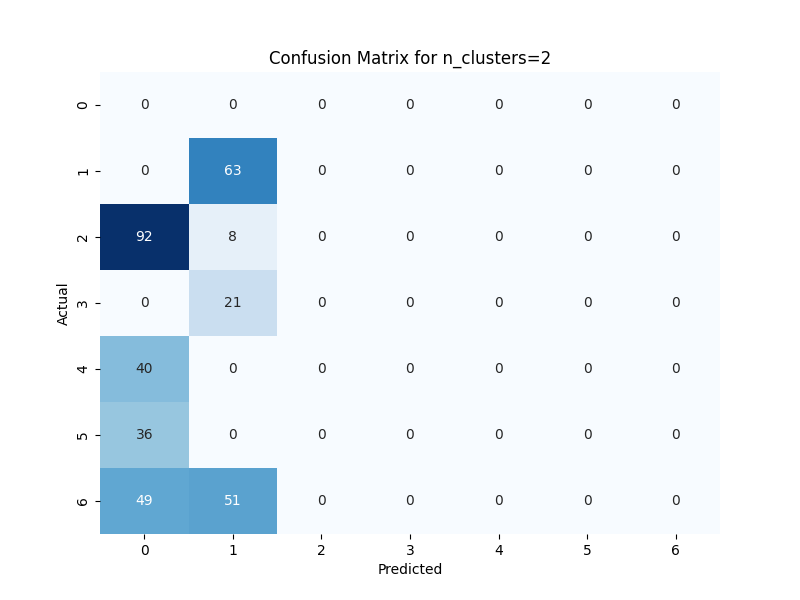
\includegraphics[width=.9\linewidth]{../K-means/Output/Dataset1/confusionMatrix_k=2.png}
			\caption{Confussion matrix for k = 2}
			\label{Dataset1ConfusionMatrixk2}
		\end{subfigure}%
		\begin{subfigure}{.5\textwidth}
			\centering
			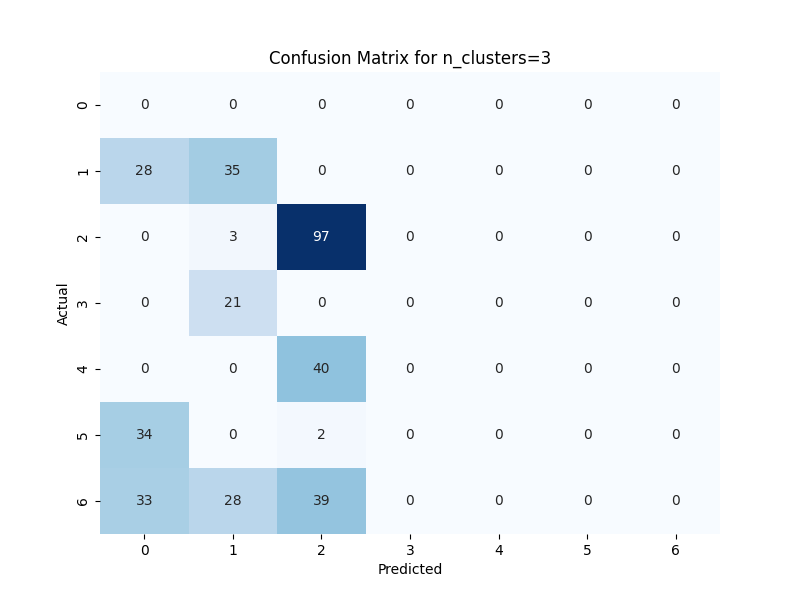
\includegraphics[width=.9\linewidth]{../K-means/Output/Dataset1/confusionMatrix_k=3.png}
			\caption{Confussion matrix for k = 2}
			\label{Dataset1ConfusionMatrixk3}
		\end{subfigure}
		\caption{Dataset 1: Scatter plot with value k = 2,3}
		\label{Dataset1ConfussionMatrix23}
	\end{figure}

	\begin{figure}[H]
		\centering
		\begin{subfigure}{.6\textwidth}
			\centering
			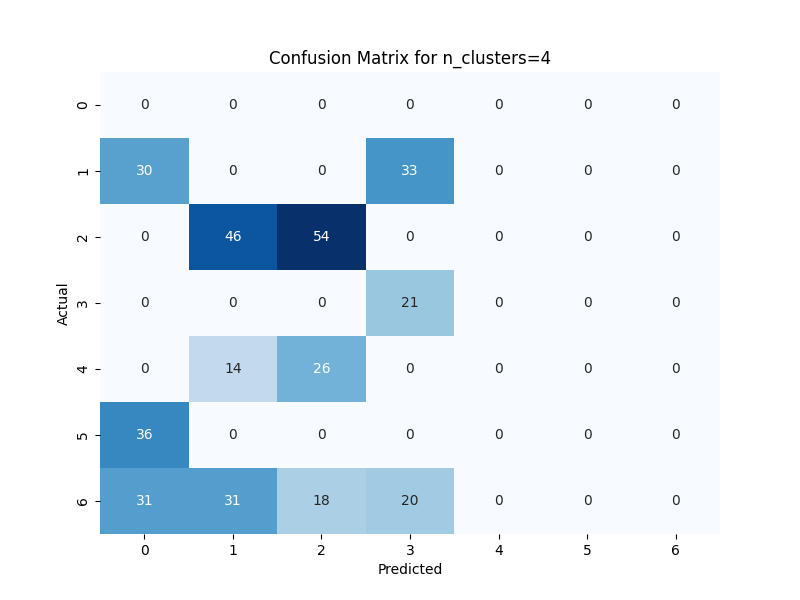
\includegraphics[width=.9\linewidth]{../K-means/Output/Dataset1/confusionMatrix_k=4.png}
			\caption{Confussion matrix for k = 4}
			\label{Dataset1ConfusionMatrixk4}
		\end{subfigure}%
		\begin{subfigure}{.6\textwidth}
			\centering
			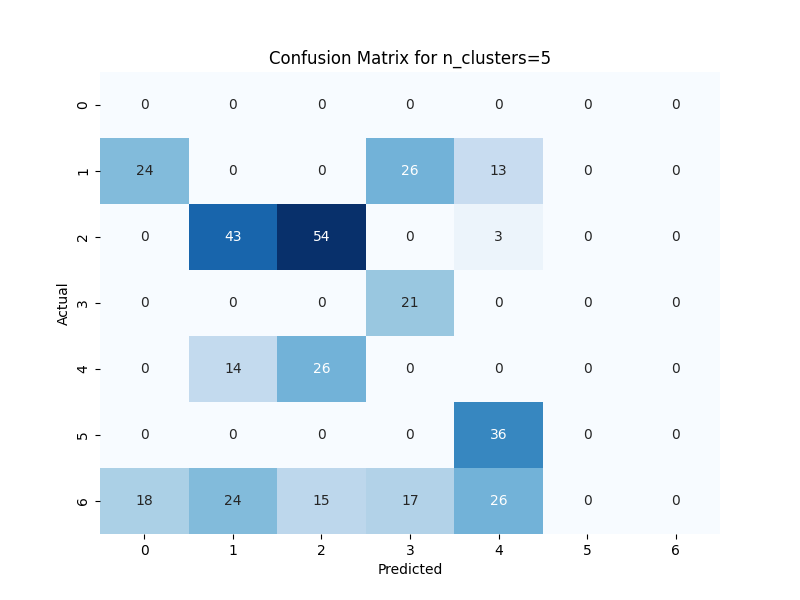
\includegraphics[width=.9\linewidth]{../K-means/Output/Dataset1/confusionMatrix_k=5.png}
			\caption{Confussion matrix for k = 5}
			\label{Dataset1ConfusionMatrixk5}
		\end{subfigure}
		\begin{subfigure}{.6\textwidth}%
			\centering
			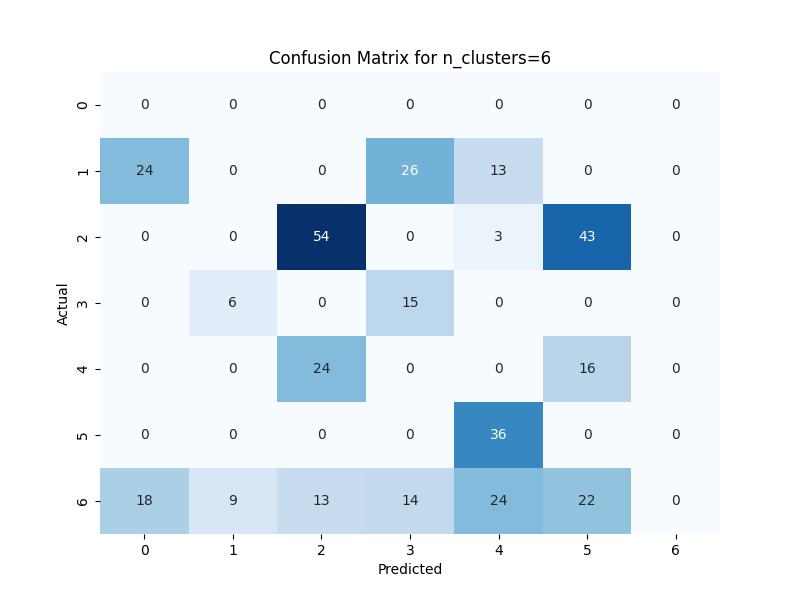
\includegraphics[width=.9\linewidth]{../K-means/Output/Dataset1/confusionMatrix_k=6.png}
			\caption{Confussion matrix for k = 6}
			\label{Dataset1ConfusionMatrixk6}
		\end{subfigure}
		\caption{Dataset 1: Scatter plot with value k = 4, 5, 6}
		\label{Dataset1ConfussionMatrix456}
	\end{figure}

	\begin{figure}[H]
		\centering
		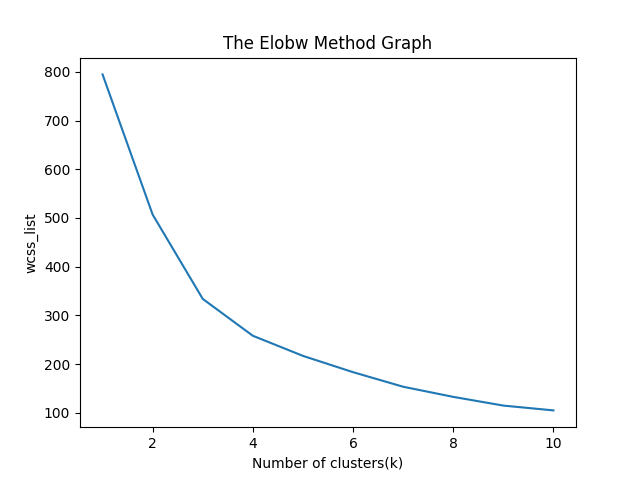
\includegraphics[scale=0.7]{../K-means/Output/Dataset1/ElbowMethod.png}
		\caption{Dataset 1 ElbowMethod output plot}
		\label{dataset1ElobowMethod}
	\end{figure}

	\begin{figure}[H]
		\centering
		\begin{subfigure}{.5\textwidth}
			\centering
			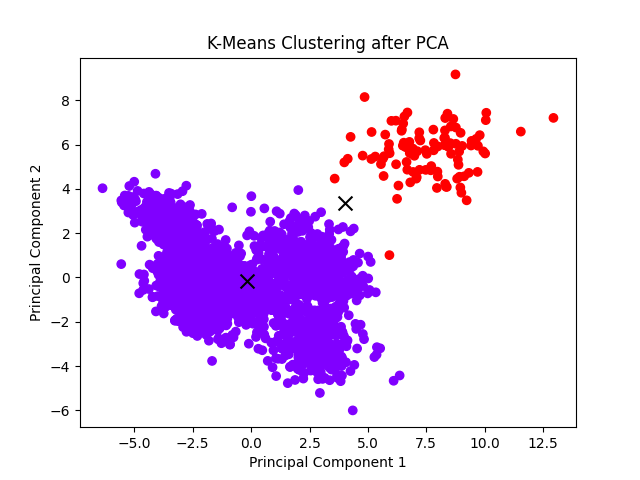
\includegraphics[width=.9\linewidth]{../K-means/Output/Dataset2/scatterPlot_k=2.png}
			\caption{Scatter plot for k = 2}
			\label{Dataset2Scatterplotk2}
		\end{subfigure}%
		\begin{subfigure}{.5\textwidth}
			\centering
			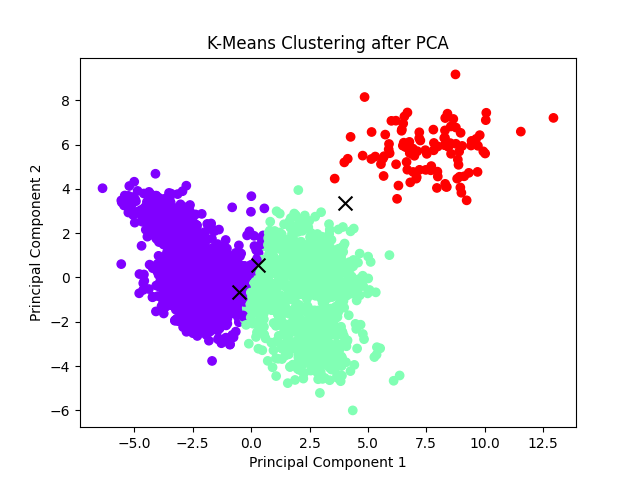
\includegraphics[width=.9\linewidth]{../K-means/Output/Dataset2/scatterPlot_k=3.png}
			\caption{Scatter plot for k = 3}
			\label{Dataset2Scatterplotk3}
		\end{subfigure}
		\caption{Dataset 2: Scatter plot with value k = 2,3}
		\label{Dataset2Scatterplot23}
	\end{figure}

	\begin{figure}[H]
		\centering
		\begin{subfigure}{.5\textwidth}
			\centering
			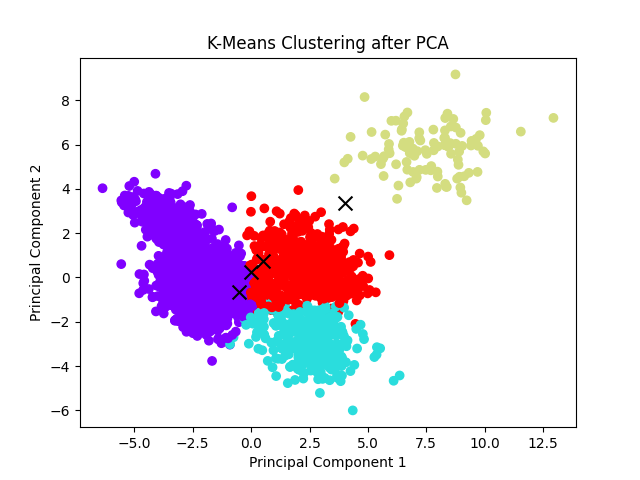
\includegraphics[width=.9\linewidth]{../K-means/Output/Dataset2/scatterPlot_k=4.png}
			\caption{Scatter plot for k = 4}
			\label{Dataset2Scatterplotk4}
		\end{subfigure}%
		\begin{subfigure}{.5\textwidth}
			\centering
			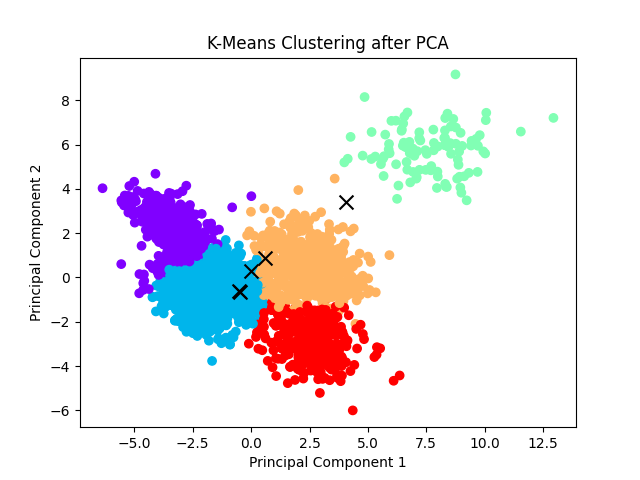
\includegraphics[width=.9\linewidth]{../K-means/Output/Dataset2/scatterPlot_k=5.png}
			\caption{Scatter plot for k = 5}
			\label{Dataset2Scatterplotk5}
		\end{subfigure}
		\begin{subfigure}{.5\textwidth}%
			\centering
			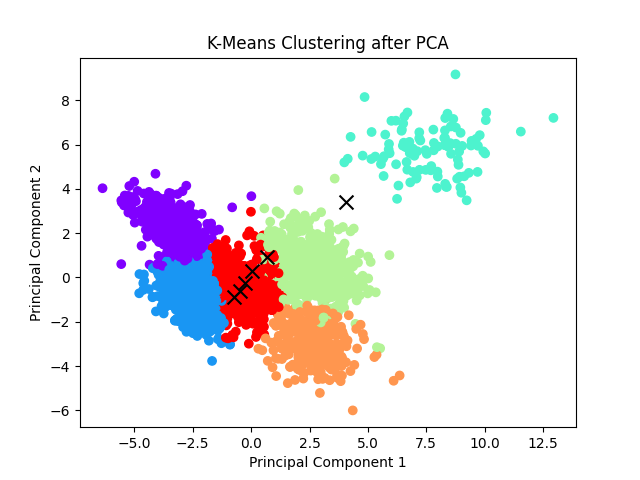
\includegraphics[width=.9\linewidth]{../K-means/Output/Dataset2/scatterPlot_k=6.png}
			\caption{Scatter plot for k = 6}
			\label{Dataset2Scatterplotk6}
		\end{subfigure}
		\caption{Dataset 2: Scatter plot with value k = 4, 5, 6}
		\label{Dataset2Scatterplot456}
	\end{figure}

	\begin{figure}[H]
		\centering
		\begin{subfigure}{.5\textwidth}
			\centering
			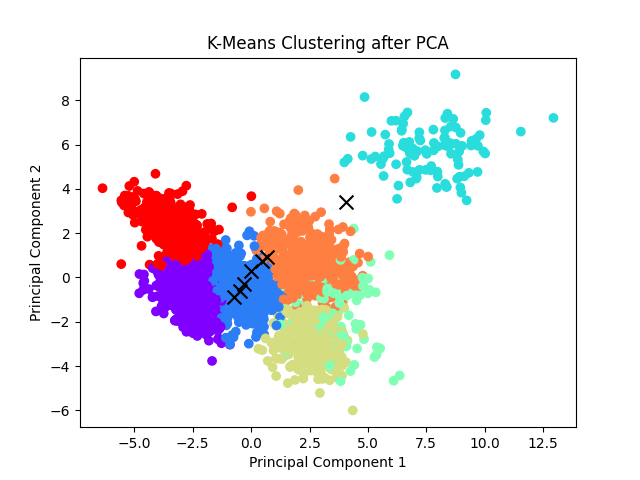
\includegraphics[width=.9\linewidth]{../K-means/Output/Dataset2/scatterPlot_k=7.png}
			\caption{Scatter plot for k = 7}
			\label{Dataset2Scatterplotk7}
		\end{subfigure}%
		\begin{subfigure}{.5\textwidth}
			\centering
			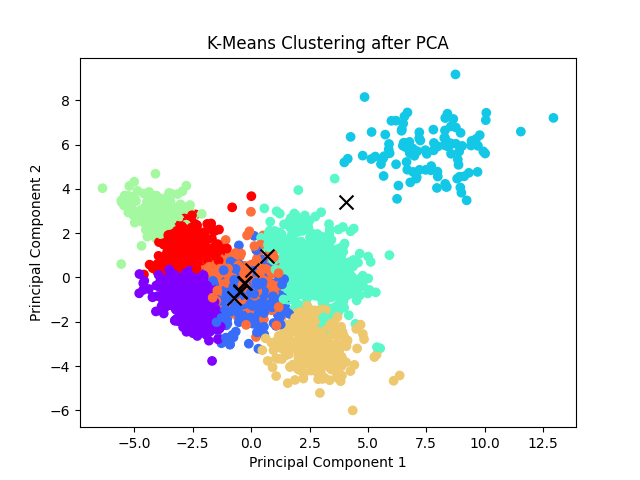
\includegraphics[width=.9\linewidth]{../K-means/Output/Dataset2/scatterPlot_k=8.png}
			\caption{Scatter plot for k = 8}
			\label{Dataset2Scatterplotk8}
		\end{subfigure}
		\caption{Dataset 2: Scatter plot with value k = 7,8}
		\label{Dataset2Scatterplot78}
	\end{figure}

	\begin{figure}[H]
		\centering
		\begin{subfigure}{.5\textwidth}
			\centering
			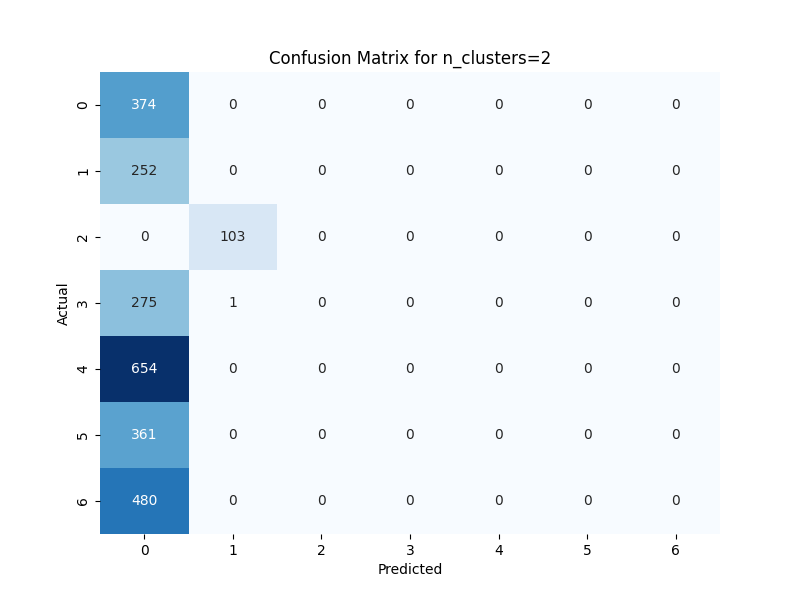
\includegraphics[width=.9\linewidth]{../K-means/Output/Dataset2/confusionMatrix_k=2.png}
			\caption{Confussion matrix for k = 2}
			\label{Dataset2ConfusionMatrixk2}
		\end{subfigure}%
		\begin{subfigure}{.5\textwidth}
			\centering
			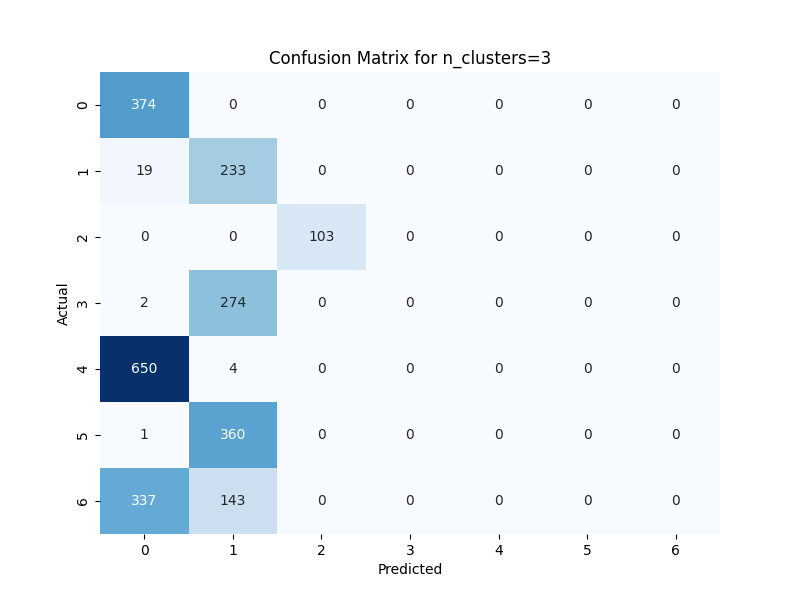
\includegraphics[width=.9\linewidth]{../K-means/Output/Dataset2/confusionMatrix_k=3.png}
			\caption{Confussion matrix for k = 2}
			\label{Dataset2ConfusionMatrixk3}
		\end{subfigure}
		\caption{Dataset 2: Scatter plot with value k = 2,3}
		\label{Dataset2ConfussionMatrix23}
	\end{figure}

	\begin{figure}[H]
		\centering
		\begin{subfigure}{.6\textwidth}
			\centering
			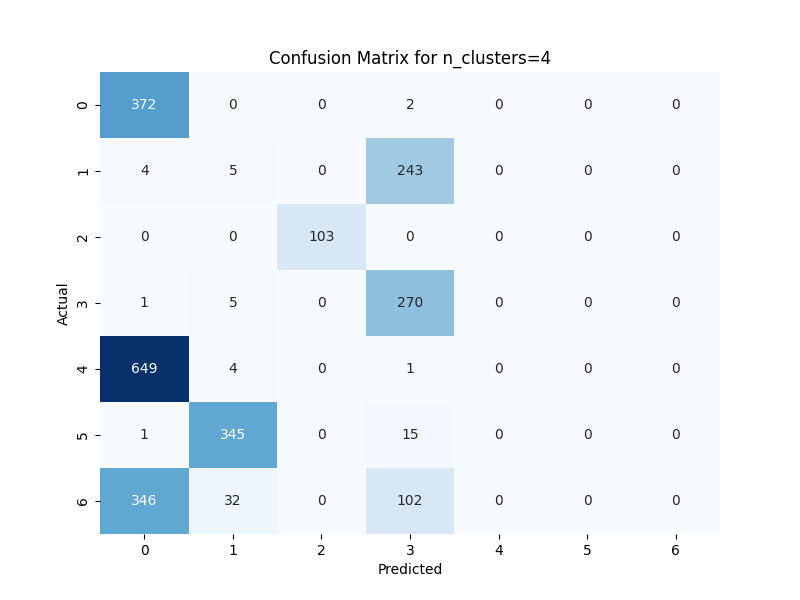
\includegraphics[width=.9\linewidth]{../K-means/Output/Dataset2/confusionMatrix_k=4.png}
			\caption{Confussion matrix for k = 4}
			\label{Dataset2ConfusionMatrixk4}
		\end{subfigure}%
		\begin{subfigure}{.6\textwidth}
			\centering
			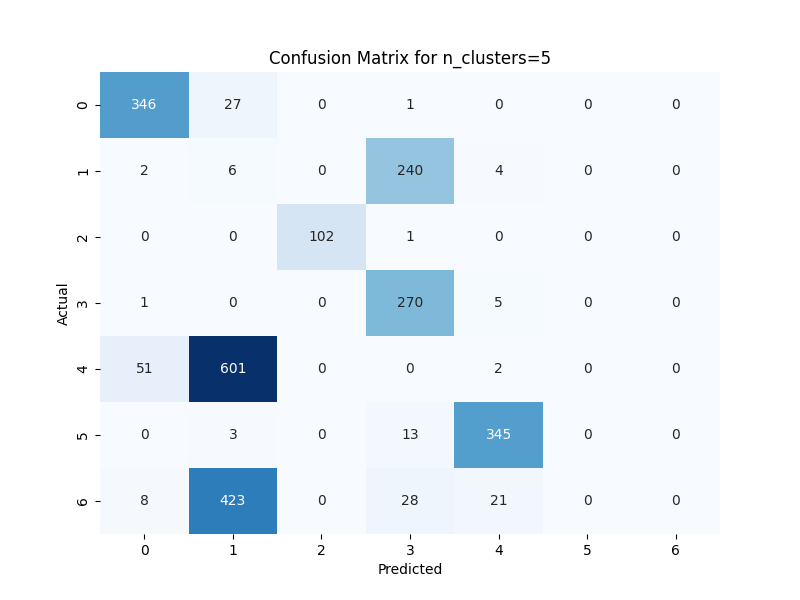
\includegraphics[width=.9\linewidth]{../K-means/Output/Dataset2/confusionMatrix_k=5.png}
			\caption{Confussion matrix for k = 5}
			\label{Dataset2ConfusionMatrixk5}
		\end{subfigure}
		\begin{subfigure}{.6\textwidth}%
			\centering
			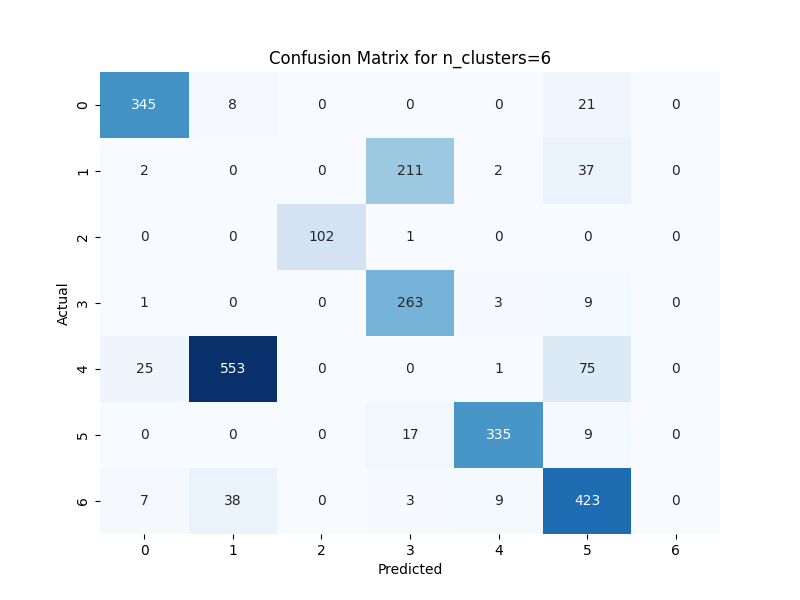
\includegraphics[width=.9\linewidth]{../K-means/Output/Dataset2/confusionMatrix_k=6.png}
			\caption{Confussion matrix for k = 6}
			\label{Dataset2ConfusionMatrixk6}
		\end{subfigure}
		\caption{Dataset 2: Scatter plot with value k = 4, 5, 6}
		\label{Dataset2ConfussionMatrix456}
	\end{figure}

	\begin{figure}[H]
		\centering
		\begin{subfigure}{.5\textwidth}
			\centering
			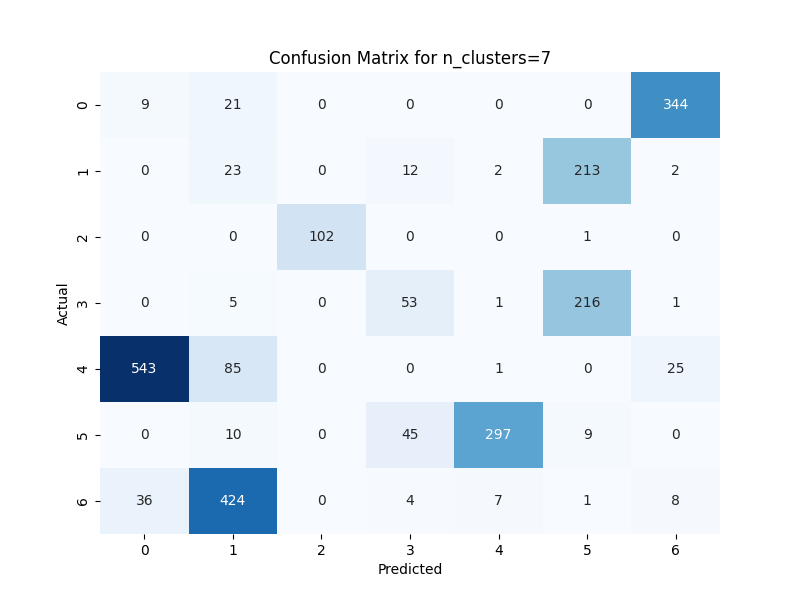
\includegraphics[width=.9\linewidth]{../K-means/Output/Dataset2/confusionMatrix_k=7.png}
			\caption{Confussion matrix for k = 7}
			\label{Dataset2ConfusionMatrixk7}
		\end{subfigure}%
		\begin{subfigure}{.5\textwidth}
			\centering
			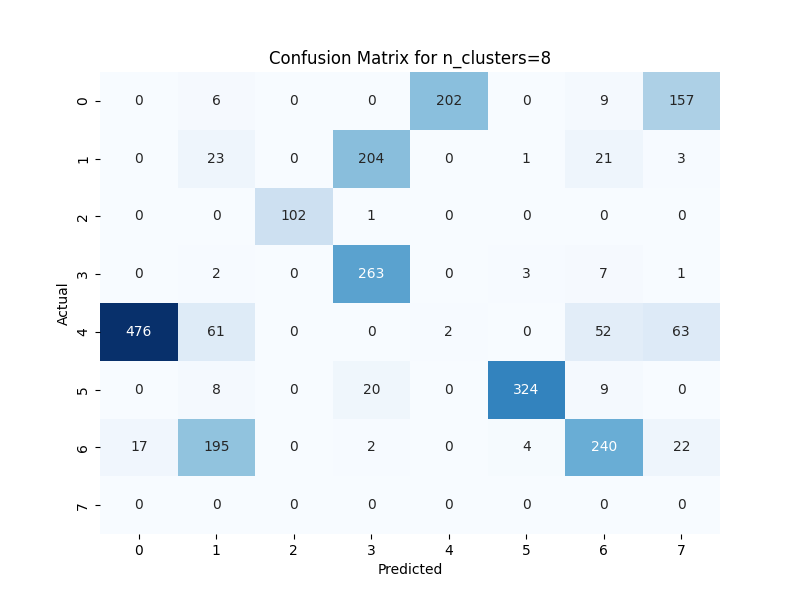
\includegraphics[width=.9\linewidth]{../K-means/Output/Dataset2/confusionMatrix_k=8.png}
			\caption{Confussion matrix for k = 8}
			\label{Dataset2ConfusionMatrixk8}
		\end{subfigure}
		\caption{Dataset 2: Scatter plot with value k = 7,8}
		\label{Dataset2ConfussionMatrix78}
	\end{figure}

	\begin{figure}[H]
		\centering
		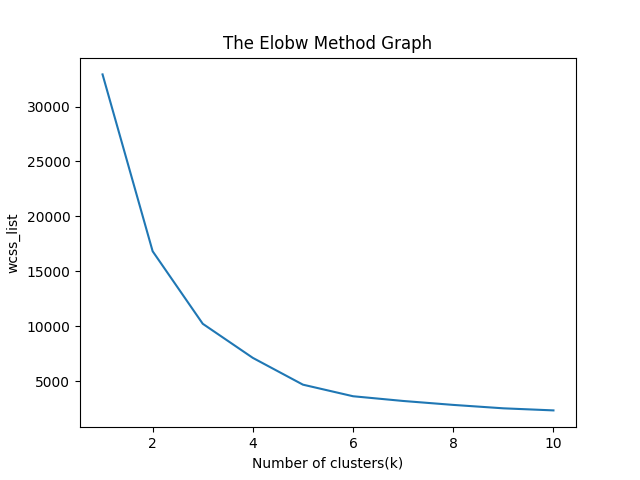
\includegraphics[scale=0.7]{../K-means/Output/Dataset2/ElbowMethod.png}
		\caption{Dataset 2 ElbowMethod output plot}
		\label{dataset2ElobowMethod}
	\end{figure}

	\newpage
	\subsection*{AHC}
	Script for this method is situated in directory AHC and the name of the script is AHC.ipynb. \\
	\\
	The dendrograms are shown in figure \ref{Dataset1Dendrograms} and figure \ref{Dataset2Dendrograms}. Distance threshold was set to visualize the different clusters that are formed from the AHC method. For dataset 1 distance threshold was set to 5 and 3 for complete linkange (figure \ref{Dataset1completeLinkage}) and UPGMA linkage (figure ref{Dataset1UPGMA}) respectively. For dataset 2 distance threshold was set to 11 and 4.1 for complete linkange (figure \ref{Dataset2completeLinkage}) and UPGMA linkage (figure \ref{Dataset2UPGMA}) respectively.\\
	\\
	\begin{table}[H]
		\centering
		\begin{tabular}{|c|c|c|c|c|c|c|}
			\hline
			Class & 1 & 2 & 3 & 4 & 5 & 6 \\
			\hline
			Data count & 63 & 100 & 21 & 40 & 36 & 100 \\
			\hline
		\end{tabular}
		\caption{Dataset 1 Amount of points for each class}
		\label{Dataset1ClassesCountTable}
	\end{table}

	\begin{table}[H]
		\centering
		\begin{tabular}{|c|c|c|c|c|c|c|c|}
			\hline
			Class & 0 & 1 & 2 & 3 & 4 & 5 & 6 \\
			\hline
			Data count & 374 & 252 & 103 & 276 & 654 & 361 & 480 \\
			\hline
		\end{tabular}
		\caption{Dataset 2 Amount of points for each class}
		\label{Dataset2ClassesCountTable}
	\end{table}

	By visual inspection of the dendrograms, for dataset 1, complete linkage is much better at representing the amount of datapoints in each clusters. Looking at table \ref{Dataset1ClassesCountTable} where it shows how many datapoints belongs to each class and comparing the complete linkage figure \ref{Dataset1completeLinkage}, the dataset is much better represented than using UPGMA. UPGMA is just assiging a big chunk of the datapoints to one class.\\
	\\
	The same conclusion can be made for dataset 2. In figure \ref{Dataset2completeLinkage} where complete linkage dendrogram is shown and table \ref{Dataset2ClassesCountTable} which shows how many datapoints belongs to each class, the dataset is much better represented than using UPGMA. The purple cluster can be the datapoints that belongs class 4, which contains the most datapoints.\\
	\\
	This method is slow, takes a lot of time to create the dendrograms espacially the complete linkage for dataset 2, take approximatly 1 minute. This method seems to be more expensive resources wise than the other methods.
	\begin{figure}[H]
		\centering
		\begin{subfigure}{.5\textwidth}
			\centering
			\includegraphics[width=.9\linewidth]{../AHC/Dendrograms/Dataset1/completeLinkage.png}
			\caption{Dataset 1 complete linkage dendrogram}
			\label{Dataset1completeLinkage}
		\end{subfigure}%
		\begin{subfigure}{.5\textwidth}
			\centering
			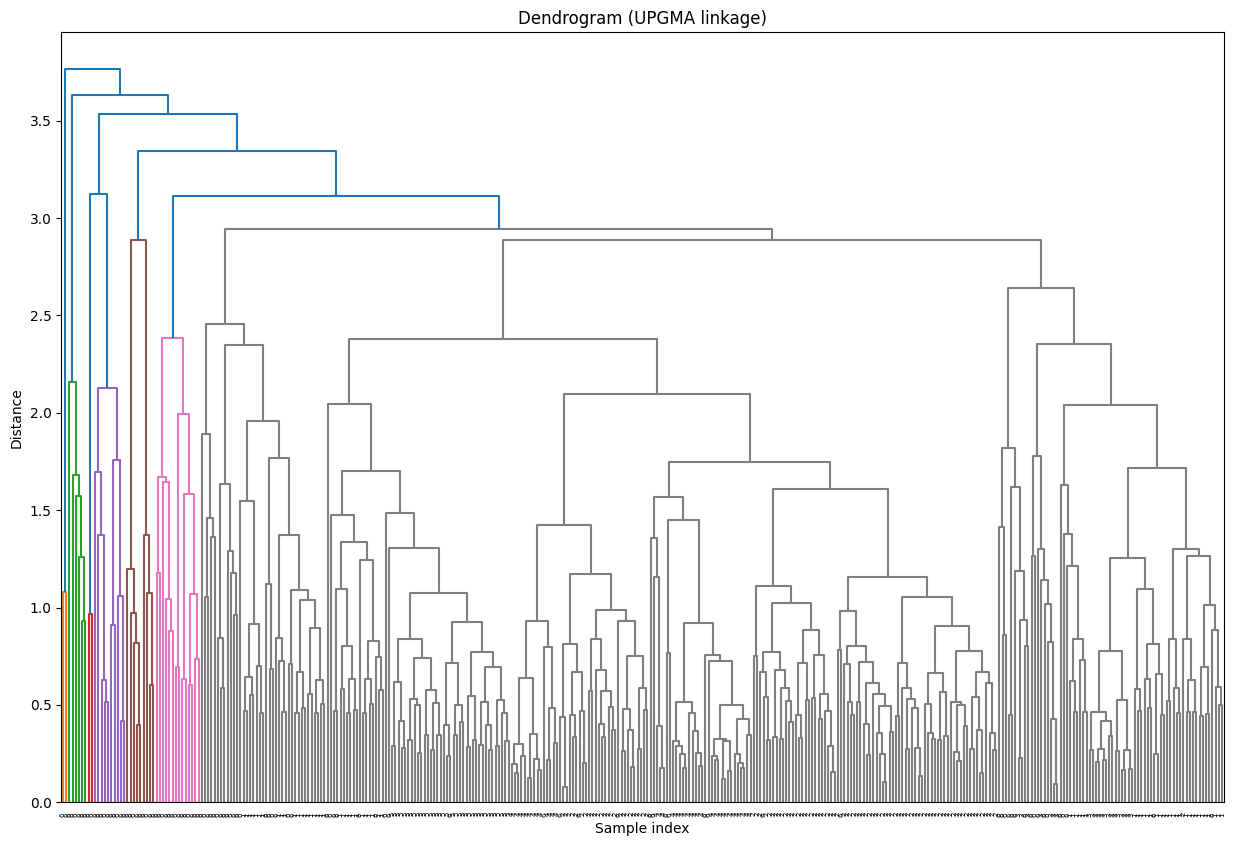
\includegraphics[width=.9\linewidth]{../AHC/Dendrograms/Dataset1/UPGMA_linkage.png}
			\caption{Dataset 1 UPGMA linkage dendrogram}
			\label{Dataset1UPGMA}
		\end{subfigure}
		\caption{Dataset 1 dendrograms}
		\label{Dataset1Dendrograms}
	\end{figure}

	\begin{figure}[H]
		\centering
		\begin{subfigure}{.5\textwidth}
			\centering
			\includegraphics[width=.9\linewidth]{../AHC/Dendrograms/Dataset2/completeLinkage.png}
			\caption{Dataset 2 complete linkage dendrogram}
			\label{Dataset2completeLinkage}
		\end{subfigure}%
		\begin{subfigure}{.5\textwidth}
			\centering
			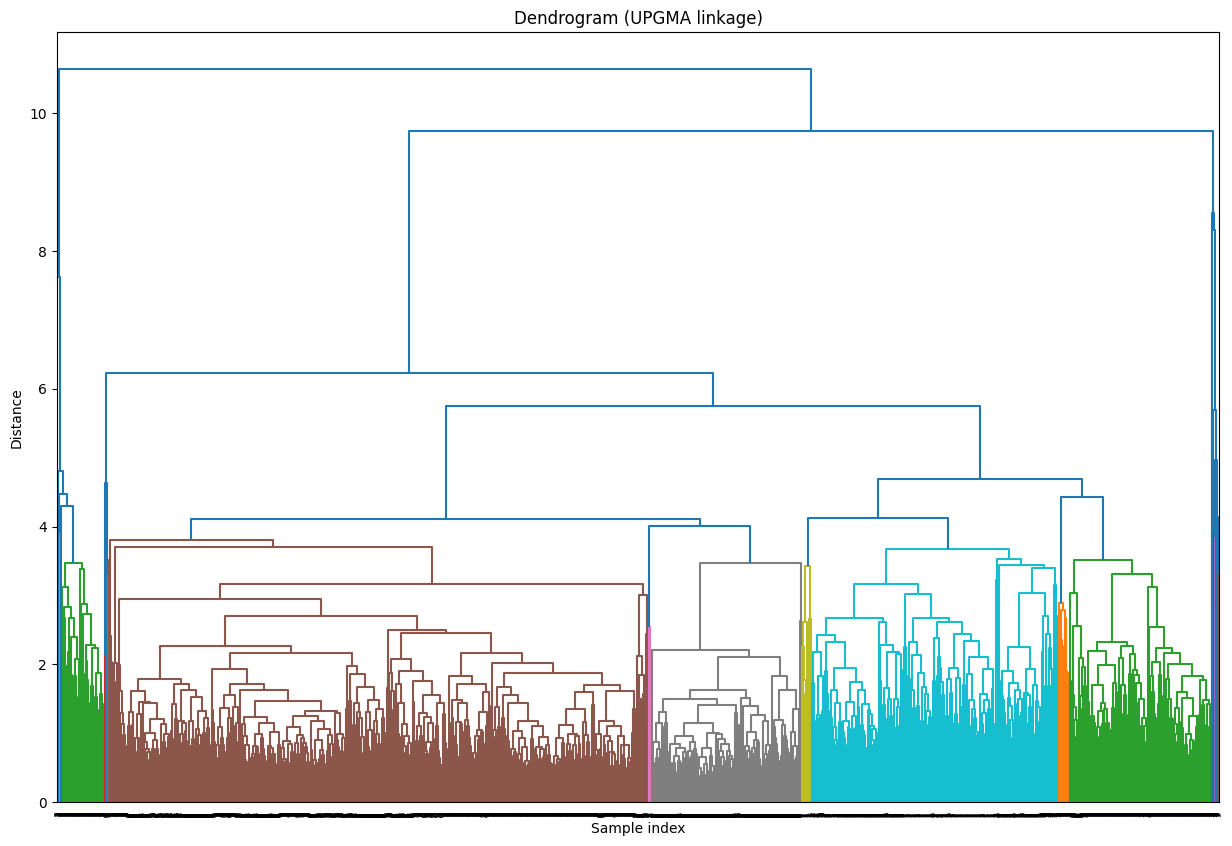
\includegraphics[width=.9\linewidth]{../AHC/Dendrograms/Dataset2/UPGMA_linkage.png}
			\caption{Dataset 2 UPGMA linkage dendrogram}
			\label{Dataset2UPGMA}
		\end{subfigure}
		\caption{Dataset 2 dendrograms}
		\label{Dataset2Dendrograms}
	\end{figure}

	\newpage
	\subsection*{SOM}	
	For dataset 1 best plot is when sigma = 0.2, learning rate = 0.5, nr of iterations = 10000.\\
	Denna gången har bara den bästa output, och sen gör en table som visar vilka parameter values jag testade
	% Do tests on different values for: number of neurons, learning rate, nr iterations, sigma value
	% Different settings: 
	% size of the map - x and y
	% learning rate
	% sigma - neighborhood function
	% heatmap - most represented class in each position 
	% plot the component planes
	\subsection*{Conclusion}
	\newpage
	Before submittion, check the script descriptions in the jupyter notebook files if they are correct and full\\
	
	Write a conclusion about the five methods, which one is best and worst, which is most efficient and so on
	\\
	Compare how the methods have classified the datasets
	\bibliographystyle{plainurl} 
	\bibliography{ref} 
\end{document}